\documentclass[a4paper,12pt]{article}   % 文檔類型為article
\usepackage{setspace}
\usepackage{fontspec}% 使用系统字体
\usepackage{xeCJK}    % 提供中文支持

% 设置中文正文字体为標楷體,你需要确保系统上有標楷體字体文件
\setCJKmainfont{標楷體}

%\onehalfspacing % 1.5 倍行距,與 Word 中的默認行距相同
%\pagestyle{empty}

\setmainfont{Times New Roman}
\fontsize{12pt}{\baselineskip}   % 設置字體大小為12pt,行距為單行


\usepackage{pdfpages}
\usepackage{enumitem}
\usepackage{fontspec}
\usepackage{authblk} 
\usepackage{titlesec}
\usepackage{amssymb}
\usepackage{graphicx}
\usepackage{titlesec}
\titlespacing{\section}{0pt}{*2}{*1}
\titlespacing{\subsection}{0pt}{*2}{*1}
\titlespacing{\subsubsection}{0pt}{*2}{*1}

\usepackage{tabularx}
\usepackage{multirow}
%\usepackage{colortbl}
\usepackage{amsthm}
\usepackage{booktabs} % 用於漂亮的表格樣式


\usepackage{colortbl} % 用於表格顏色
\usepackage{xcolor}   % 用於文本顏色
\definecolor{lightgray}{gray}{0.9} % 自定義顏色
\newcommand{\xq}[1]{\textcolor{red}{#1}}

\pagestyle{plain}


\begin{document}
%\maketitle

\begin{center}
	{\fontsize{16pt}{12pt}\selectfont Text Sentiment Classification with Prompt Learning}
	
\end{center}

\hfill  B092040016 陳昱逢
	
	
\begin{center}
	Assignment 6
\end{center}

\section{Task 1}
	任務一分別測試了 BERT 和 RoBERTa 兩個模型。此任務首先採取預訓練好的模型直接 fine-tune 在 sentiment classification 的 task 上,我最後採用的模型為 RoBERTa-large 並在進入最後一層前加了 Dropout 來防止模型過擬合。Table\ \ref{table:comparison_task1} 顯示了訓練 Epoch 為 5 的測試集結果。
	
\begin{table}[htb]
	\centering	
	\normalsize
    \caption{Simulation results of sentiment classification on Twitter US Airline}
    \vspace{0.15\baselineskip}
    \begin{tabularx}{1\textwidth}{@{}XX@{}}
		\toprule
		\textbf{Model} & \textbf{Accuracy} \\
		\midrule
		BERT     &  0.8392  \\ 
		RoBERTa-base  & 0.8532 \\
		RoBERTa-large + Dropout & \textbf{0.8652} \\
		\bottomrule
	\end{tabularx}
	\label{table:comparison_task1}
    \vspace{0.15\baselineskip}
\end{table}

為了再提升準確度,我訓練更久,Epoch 為 15,隨後利用ensemble的概念,選取5個model做權重投票投出結果,發現可以再有些微的提升。Table\ \ref{table:comparison_task1_2} 呈現測試集結果。

\begin{table}[htb]
	\centering	
	\normalsize
    \caption{Simulation results of sentiment classification on Twitter US Airline}
    \vspace{0.15\baselineskip}
    \begin{tabularx}{1\textwidth}{@{}XX@{}}
		\toprule
		\textbf{Model} & \textbf{Accuracy} \\
		\midrule
		RoBERTa-large + Dropout & 0.8717 \\
		RoBERTa-large + Dropout + ensemble & \textbf{0.8722} \\
		\bottomrule
	\end{tabularx}
	\label{table:comparison_task1_2}
    \vspace{0.15\baselineskip}
\end{table}



\iffalse
\begin{table}[htb]
	\centering	
	\normalsize
    \newcommand{\z}{\phantom{0}}
    \caption{configurations of my experiment}
    \vspace{0.15\baselineskip}
    \resizebox{0.6\textwidth}{!}{
		\begin{tabular}[c]{|l|l|}
			\hline
			\textbf{parameter} & \textbf{configuration} \\
			\hline
			num\_epochs   &  45 \\
			\hline
			decay\_epochs & 15 \\
			\hline
			init\_lr & 0.01  \\
			\hline
			AdamW & weight\_decay = 0.01 \\
    			\hline
		\end{tabular}
	}
	\label{table:param}
   \vspace{0.1\baselineskip}
\end{table}
\fi


\section{Task 2}

	任務二嘗試了三種不同的 template 並實驗於 zero-shot, one-shot and few-shot 三種情況中。Table\ \ref{table:template_prompts} 呈現我此次實驗不同 template 的設定。

\begin{table}[htb]
	\centering	
	\normalsize
    \caption{Manuallly designed template}
    \vspace{0.15\baselineskip}
    \begin{tabularx}{1\textwidth}{@{}l|l@{}}
		\toprule
		\textbf{Template} & \textbf{Prompt} \\
		\midrule
		Template 1   & It is \textbf{[MASK]}. \\
		Template 2   & The sentiment of this sentence is \textbf{[MASK]}. \\
		Template 3   & How do you feel after reading this sentence? I feel \textbf{[MASK]}.  \\  % 改成 how 試試看
		\bottomrule
	\end{tabularx}
	\label{table:template_prompts}
    \vspace{0.15\baselineskip}
\end{table}

\begin{figure}[htb]
  \vspace{0.1\baselineskip}  
  \centering  
  %\begin{center}
    \resizebox{1\textwidth}{!}{\includegraphics{one_shot.jpg}}
    \caption{one-shot prompts for different templates}
    \label{fig:one_shot}
  %\end{center}
  \vspace{0.1\baselineskip}
\end{figure}	


\subsection{zero-shot}

	Table\ \ref{table:zero_shot} 呈現不同 template 在 zero-shot 情況下的實驗結果。

\vspace{-5mm}
\begin{table}[htb]
	\centering	
	\normalsize
    \newcommand{\z}{\phantom{0}}
    \caption{Simulation results of zero-shot with different templates}
    \vspace{0.15\baselineskip}
    %\resizebox{0.5\textwidth}{!}{
	\begin{tabularx}{1\textwidth}{@{}l*{4}{>{\centering\arraybackslash}X}@{}}\toprule
		\textbf{Template} & \textbf{Accuracy} & \textbf{Precision} & \textbf{Recall} & \textbf{F1 score}\\
		%\hline
		\midrule
		Template 1           & \textbf{0.4255}       & \textbf{0.6375}     & \textbf{0.4255}       & \textbf{0.4236}  \\ 
		Template 2           & 0.2175                & 0.6013              & 0.2175                & 0.1504  \\
		Template 3           & 0.1616                & 0.4440              & 0.1616                & 0.0453  \\
    		\bottomrule
	\end{tabularx}
	%}
	\label{table:zero_shot}
   \vspace{-\baselineskip}
\end{table}





\subsection{one-shot}
	
	Figure\ \ref{fig:one_shot} 展示我此次實驗針對不同 template 設定的 one-shot 範例提示。Table\ \ref{table:one_shot} 呈現不同 template 在 one-shot 情況下的實驗結果。

\vspace{-5mm}
\begin{table}[htb]
	\centering	
	\normalsize
    \newcommand{\z}{\phantom{0}}
    \caption{Simulation results of one-shot with different templates}
    \vspace{0.15\baselineskip}
    %\resizebox{0.5\textwidth}{!}{
	\begin{tabularx}{1\textwidth}{@{}l*{4}{>{\centering\arraybackslash}X}@{}}\toprule
		\textbf{Template} & \textbf{Accuracy} & \textbf{Precision} & \textbf{Recall} & \textbf{F1 score}\\
		%\hline
		\midrule
		Template 1           & \textbf{0.3740}       & \textbf{0.5388}      & \textbf{0.3740}       & \textbf{0.3667}  \\ 
		Template 2           & 0.1614                & 0.0260               & 0.1614                & 0.0449  \\
		Template 3           & 0.1614                & 0.0260               & 0.1614                & 0.0449  \\
    		\bottomrule
	\end{tabularx}
	%}
	\label{table:one_shot}
   \vspace{-\baselineskip}
\end{table}



\subsection{few-shot}

	Few-shot 則從訓練資料裡多拿幾個樣本來當做 prompt,我拿了三個樣本,主要想法是每一個類別都拿一個樣本。Table\ \ref{table:few_shot} 呈現不同 template 在 few-shot 情況下的實驗結果。


\begin{table}[htb]
	\centering	
	\normalsize
    \newcommand{\z}{\phantom{0}}
    \caption{Simulation results of few-shot with different templates}
    \vspace{0.15\baselineskip}
    %\resizebox{0.5\textwidth}{!}{
	\begin{tabularx}{1\textwidth}{@{}l*{4}{>{\centering\arraybackslash}X}@{}}\toprule
		\textbf{Template} & \textbf{Accuracy} & \textbf{Precision} & \textbf{Recall} & \textbf{F1 score}\\
		%\hline
		\midrule
		Template 1           & \textbf{0.6270}       & 0.3931              & \textbf{0.6270}       & \textbf{0.4832}  \\ 
		Template 2           & 0.2631                & 0.5826              & 0.2631                & 0.2269  \\
		Template 3           & 0.3198                & \textbf{0.6115}     & 0.3198                & 0.3038  \\
    		\bottomrule
	\end{tabularx}
	%}
	\label{table:few_shot}
   \vspace{-\baselineskip}
\end{table}





\section{Task 3}

	任務三實驗不同的手動 template 設定以及不同數量的 demonstration 的表現度。Table\ \ref{table:manually_crafted_template} 呈現了三種不同的手動 template 的設定。
	
\begin{table}[htb]
	\centering	
	
    \caption{Manuallly crafted template}
    \vspace{0.15\baselineskip}
    \footnotesize
    \begin{tabularx}{1.15\textwidth}{@{}l|l@{}}
		\toprule
		\textbf{Template} & \textbf{Prompt} \\
		\midrule
		Manual Template 1   &  \{" placeholder":"text\_a"\} It was \{"mask"\}. \\
		Manual Template 2   & \{"placeholder":"text\_a"\} The sentiment of this sentence is \{"mask"\}. \\
		Manual Template 3   & \{"placeholder":"text\_a"\} How do you feel after reading this sentence? I feel \{"mask"\}.  \\  
		\bottomrule
	\end{tabularx}
	\label{table:manually_crafted_template}
    \vspace{0.1\baselineskip}
\end{table}

\subsection{Different manually crafted templates}
	
	Table\ \ref{table:different_manually_templates} 比較了三種不同的手動 template 以及自動產生 template 的表現度,由結果可以觀察出自動生成 template 的表現效果達到最好。
	
\vspace{-5mm}
\begin{table}[htb]
	\centering	
	\normalsize
    \caption{Performance comparison of different manually templates}
    \vspace{0.15\baselineskip}
    \begin{tabularx}{1\textwidth}{@{}XX@{}}
		\toprule
		\textbf{Template} & \textbf{accuracy} \\
		\midrule
		Manual Template 1       &  0.6918  \\ 
		Manual Template 2       &  0.8623  \\
		Manual Template 3       &  0.7770  \\ 
		Auto-generate Template  & \textbf{0.9082} \\
		\bottomrule
	\end{tabularx}
	\label{table:different_manually_templates}
    \vspace{0.15\baselineskip}
\end{table}


\vspace{-2mm}
\subsection{Differenet numbers of demonstrations}

Table\ \ref{table:different_demonstrations} 比較了不同數量的 demonstrations 對模型表現度的影響,由結果可以觀察出 使用 6 個數量的 demonstration 結果較好。以下每一段分別匯報對不同數量的 demonstration,最好的 template 跟 verbalizer。


\begin{table}[htb]
	\centering
	\normalsize
    \caption{Performace comparison of different numbers of demonstrations}
    \vspace{0.15\baselineskip}
    \begin{tabularx}{1\textwidth}{@{}XX@{}}
		\toprule
		\textbf{\# of demonstraions} & \textbf{accuracy} \\
		\midrule
		1        &  0.9082  \\ 
		6        &  \textbf{0.9131}  \\
		8       &   0.9066  \\ 
		\bottomrule
	\end{tabularx}
	\label{table:different_demonstrations}
    \vspace{0.15\baselineskip}
\end{table}

對於 num\_ of \_ demonstration 為 1, best template 為 \xq{\{"placeholder": "text\_a"\} It was \{"mask"\} . flat.nothing happens , and it happens to flat characters . It was terrible. a crisp psychological drama (and) a fascinating little thriller that would have been perfect for an old `` twilight zone '' episode . It was great.},而 best verbalizer 為 \xq{['horrifying', 'terrifying']} 


對於 num\_ of \_ demonstration 為 6, best template 為 \xq{\{"placeholder": "text\_a"\} It was \{"mask"\} . it was terrible.just a collection of this and that -- whatever fills time -- with no unified whole . It was terrible. serious movie-goers embarking upon this journey will find that the road to perdition leads to a satisfying destination . It was great. in that setting , their struggle is simply too ludicrous and borderline insulting . It was terrible. shyamalan takes a potentially trite and overused concept (aliens come to earth) and infuses it into a rustic , realistic , and altogether creepy tale of hidden invasion . It was great. nothing happens , and it happens to flat characters . It was terrible. serious movie-goers embarking upon this journey will find that the road to perdition leads to a satisfying destination . It was great. often lingers just as long on the irrelevant as on the engaging , which gradually turns what time is it there ? It was terrible. my big fat greek wedding is not only the best date movie of the year , it 's also a -- dare i say it twice -- delightfully charming -- and totally american , i might add -- slice of comedic bliss . It was great. the big finish is a bit like getting all excited about a chocolate eclair and then biting into it and finding the filling missing . It was terrible. a haunting tale of murder and mayhem . It was great. the plot is nothing but boilerplate clichés from start to finish , and the script assumes that not only would subtlety be lost on the target audience , but that it 's also too stupid to realize that they 've already seen this exact same movie a hundred times It was terrible. the filmmakers ' eye for detail and the high standards of performance convey a strong sense of the girls ' environment . It was great.},而 best verbalizer 為 \xq{['awful', 'good']} 


對於 num\_ of \_ demonstration 為 8, best template 為
\xq{\{"placeholder": "text\_a"\} It was \{"mask"\} ..a rude black comedy about the catalytic effect a holy fool has upon those around him in the cutthroat world of children 's television . It was terrible. a crisp psychological drama (and) a fascinating little thriller that would have been perfect for an old `` twilight zone '' episode . It was great. as lively an account as seinfeld is deadpan . It was terrible. sweet and memorable film . It was great. just a collection of this and that -- whatever fills time -- with no unified whole . It was terrible. the film jolts the laughs from the audience -- as if by cattle prod . It was great. just because a walk to remember is shrewd enough to activate girlish tear ducts does n't mean it 's good enough for our girls . It was terrible. (ramsay) visually transforms the dreary expanse of dead-end distaste the characters inhabit into a poem of art , music and metaphor . It was great. so we got ten little indians meets friday the 13th by way of clean and sober , filmed on the set of carpenter 's the thing and loaded with actors you 're most likely to find on the next inevitable incarnation of the love boat . It was terrible. diggs and lathan are among the chief reasons brown sugar is such a sweet and sexy film . It was great. as lively an account as seinfeld is deadpan . It was terrible. a crisp psychological drama (and) a fascinating little thriller that would have been perfect for an old `` twilight zone '' episode . It was great. often lingers just as long on the irrelevant as on the engaging , which gradually turns what time is it there ? It was terrible. sweet and memorable film . It was great. but it would be better to wait for the video . It was terrible. (ramsay) visually transforms the dreary expanse of dead-end distaste the characters inhabit into a poem of art , music and metaphor . It was great.},而 best verbalizer 為 \xq{['well', 'tremendous']}

\noindent Figure\ \ref{fig:demo} 呈現不同數量的 demonstrations 的準確度。

\begin{figure}[htb]
  \vspace{0.1\baselineskip}  
  \centering  
  %\begin{center}
    \resizebox{0.6\textwidth}{!}{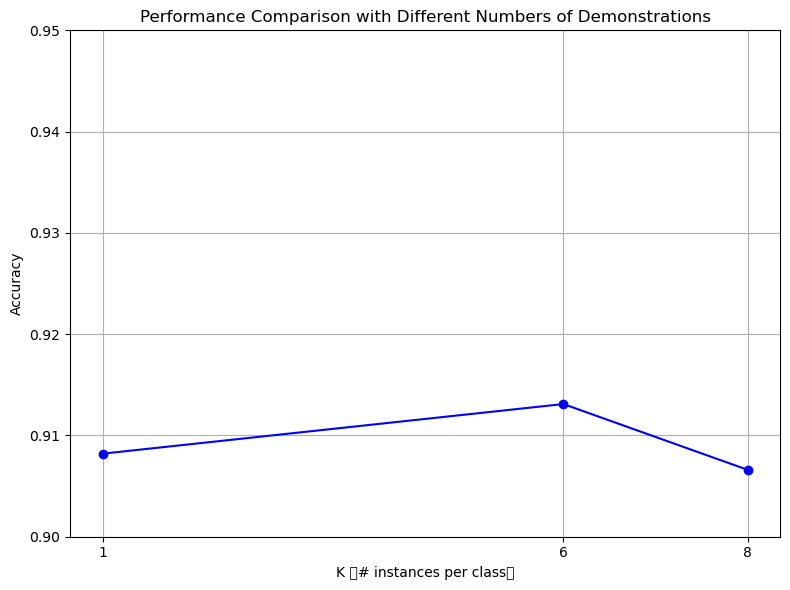
\includegraphics{draw.png}}
    \caption{LM-BFF for different numbers of demonstrations (\# instances per class)}
    \label{fig:demo}
  %\end{center}
  \vspace{0.1\baselineskip}
\end{figure}	





\end{document}